\documentclass[runningheads,a4paper]{llncs}

\usepackage{amssymb}
\setcounter{tocdepth}{3}
\usepackage{graphicx}
\usepackage{tikz}
\usepackage[T1]{fontenc}
\usepackage[scaled]{beramono}
\usepackage{listings}
\usepackage{color}
\usetikzlibrary{arrows,chains,positioning,scopes,quotes,calc}

\newcommand{\keywords}[1]{\par\addvspace\baselineskip
\noindent\keywordname\endspace\ignorespaces#1}
\pagestyle{plain}
\setlength\parindent{0pt}

\definecolor{mygreen}{RGB}{28,172,0} % color values Red, Green, Blue
\definecolor{mylilas}{RGB}{170,55,241}

\newcommand*{\StrikeThruDistance}{0.15cm}%
\newcommand*{\StrikeThru}{\StrikeThruDistance,\StrikeThruDistance}%

\tikzset{strike thru arrow/.style={
    decoration={markings, mark=at position 0.5 with {
        \draw [blue, thick,-] 
            ++ (-\StrikeThruDistance,-\StrikeThruDistance) 
            -- ( \StrikeThruDistance, \StrikeThruDistance);}
    },
    postaction={decorate},
}}

\lstset{
  language=Python,
  showstringspaces=false,
  formfeed=\newpage,
  tabsize=4,
  commentstyle=\itshape,
  basicstyle=\ttfamily,
  morekeywords={models, lambda, forms}
}

\begin{document}
\def \SystemName {Worlds} % Lol because this shit probably will change.

\mainmatter  % start of an individual contribution

% This needs some work, big time.
\title{\SystemName: A distributed MMO}

\author{Ryan Walker\\
				ryan.cjw@gmail.com}

\institute{} %Merp

\maketitle

% - Abstract:  Why, What, How 

% Worlds
%  - Overview
%  - Action Ledger
%  - Transport Hash
%  - Forward Transport hash
%  - World Tranfer
%  - Player Genesis
%  
% Trust
%  - Action ledger traceback
%  - World disconnect

\begin{abstract}
A protocol defining how anyone can join or contribute to a completely unbounded universe could allow the flexibility to organically grow an MMO faster and more efficiently then any proprietary closed system. This paper will overview a truly limitless protocol that allows developers to bolt their code into in common universe. 
\end{abstract}

\section{Introduction}
For an open software ecosystem to grow organically there should be outlets for contribution. In the context of a massively multiplayer online game the outlets become more complicated then a simple code repository. Fair game mechanics are built on a fragile ecosystem that could have negative consequences if managed improperly. The fairness and security of the game are entirely dependent on the network forming consensus on what is considered to be the truth. This is trivially done with conventional methods. A server maintains a secure connection with a player and the player pipes his actions to the server. The server then provides ground truth for the network. Distributed systems require a very different approach. Blockchains present clear deficiencies, they are too slow and the chain would get too large. A completely alternate consensus method will now be presented...

\section{Worlds}
\subsection{Overview}
A world, defined as $w_k$, is a node that forms consensus among it's own domain. It's possible for any node in the network to be a world. A world can have up to four adjacent worlds determined by itself. Players, defined as $P_k$, can enter a world one of three ways, the first being a \textbf{player genesis}(\ref{PG}). The second being a \textbf{world transfer} (\ref{WT}). The third and final method is by issuing a \textbf{refuge package}(\ref{RP}). Worlds and players both have their own RSA key pair. 

\subsection{Action Ledger}
\label{AL}
An action ledger, defined as $AL(P_{k}, w_k)$, is a chronological list of all the signed actions and reactions that has happened to a player in a world. In order to commit an action a player must concatenate current unix time with the action, then sign and sent to the world. If the action is legal, it is entered into the world's action ledger for that player. If reactions are to occur to a player, the world must concatenate current unix time with the reaction then sign and sent to the player. Players are required to keep their actions ledger dating back to their genesis, worlds are only required to keep \textbf{transport hashes} (\ref{TH}).

\subsection{Transport Hash}
\label{TH}
A transport hash is a hash of an action ledger, $h_s(AL(P_{k}, w_k))$, these are secured by the worlds and are used to prove a player is presenting an honest action ledger. The transport hash is formed when a player leaves the world. A \textbf{Forward Transport Hash} is just a transport hash kept in a special location. This is explained more in the world transfer section, it is defined as  $h_{sf}(AL(P_{k}, w_k))$

\subsection{World Transfer} 
\label{WT}
A detailed state machine outlines how players can move about neighboring worlds. Honest worlds must follow this procedure to maintain fairness, if they misbehave they could be risking a \textbf{World Disconnect} (\ref{WD}) from their neighboring worlds. 
\\
\\
\textbf{Eg:} Lets say a player, defined as $P_1$, wants to move from $w_1$ to $w_2$ (Figure \ref{w1tow2}) and then to $w_3$, The network values in this scenario are defined as...

\begin{figure}
\caption{$P_1$ moving from $w_1$ to $w_2$}
\label{w1tow2}
\begin{center}
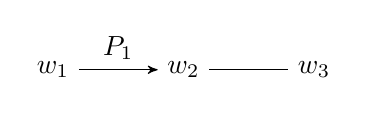
\begin{tikzpicture}[>=stealth']
{[start chain]
\node[on chain] (A) {$w_1$};
\node[on chain,join=by {->,"$P_1$"},right=of A] (B) {$w_2$};
\node[on chain,join=by {-},right=of B] (C) {$w_3$};}
\end{tikzpicture}
\end{center}
\begin{center}
\begin{tabular}{ c|c c c }
& $w_1$ & $w_2$ & $w_3$ \\
\hline 
$h_s(AL(P_1,w_k))$ & $NULL$ & $NULL$ & $NULL$ \\ 
$h_{sf}(AL(P_1,w_k))$ & $NULL$ & $NULL$ & $NULL$ \\ 
Neighbor & $w_2$ & $w_1$ \& $w_3$ & $w_2$\\
\end{tabular}
\end{center}
\end{figure}

\begin{enumerate}
\item $P_1$ sends a signed world entry packet to $w_2$
\item $w_2$ insures that $w_1$ is adjasent to itself
\item $w_2$ must verify that $P_1$ currently resides in $w_1$, this is done by ensuring $h_{sf}(AL(P_1,w_k)) = NULL$. This is found by sending a signed data request to $w_1$ 
\item $P_1$ presents $AL(P_1,w_1)$ to $w_2$
\item $w_1$ calculates $h_s(AL(P_1,w_1))$ using the $AL$ on the serverside
\item $w_2$ calculates $h_s(AL(P_1,w_1))$ using the $AL$ provided by $P_1$, the hashes must match
\item (Optional) An \textbf{Action Ledger Traceback} (\ref{ALT}) can be complete
\item $P_1$ is now granted access to $w_2$ and can submit actions
\item $w_1$ must store $h_s(AL(P_1,w_1))$, $AL(P_1,w_1)$ can be deleted
\end{enumerate}

\begin{figure}
\caption{$P_1$ in $w_2$}
\begin{center}
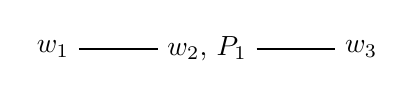
\begin{tikzpicture}[>=stealth']
{[start chain]
\node[on chain] (A) {$w_1$};
\node[on chain,join=by {-},right=of A] (B) {$w_2$, $P_1$};
\node[on chain,join=by {-},right=of B] (C) {$w_3$};}
\end{tikzpicture}
\end{center}
\begin{center}
\begin{tabular}{ c|c c c }
& $w_1$ & $w_2$ & $w_3$ \\
\hline 
$h_s(AL(P_1,w_k))$ & $ h_s(AL(P_1,w_1))$ & $NULL$ & $NULL$ \\ 
$h_{sf}(AL(P_1,w_k))$ & $NULL$ & $NULL$ & $NULL$ \\ 
Neighbor & $w_2$ & $w_1$ \& $w_3$ & $w_2$\\
\end{tabular}
\end{center}
\end{figure}

\begin{figure}
\caption{$P_1$ in $w_3$}
\begin{center}
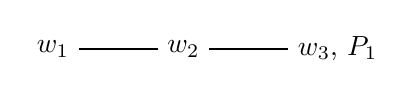
\begin{tikzpicture}[>=stealth']
{[start chain]
\node[on chain] (A) {$w_1$};
\node[on chain,join=by {-},right=of A] (B) {$w_2$};
\node[on chain,join=by {-},right=of B] (C) {$w_3$, $P_1$};}
\end{tikzpicture}
\end{center}
\begin{center}
\begin{tabular}{ c|c c c }
& $w_1$ & $w_2$ & $w_3$ \\
\hline 
$h_s(AL(P_1,w_k))$ & $h_s(AL(P_1,w_1))$ & $h_s(AL(P_1,w_2))$ & $NULL$ \\ 
$h_{sf}(AL(P_1,w_k))$ & $h_s(AL(P_1,w_2))$ & $NULL$ & $NULL$ \\ 
Neighbor & $w_2$ & $w_1$ \& $w_3$ & $w_2$\\
\end{tabular}
\end{center}
\end{figure}

\subsection{Player Genesis} 
\label{PG}
Player Genesis is the creation of a new player, for this to occur a player must digitally sign a genesis package with the current nuance of the world. The world must ensure there are no existing values entered for that player. The player is then instated into the world with all the initial player values set to zero. 

\subsection{Refuge Package}
\label{RP}
A refugee

\section{Worlds Engine Mechanics} 
The system is not entirely trustless, the neighboring worlds need to trust each other. It's possible for neighboring worlds to have disagreements and still function. For instance, $w_1$ might introduce an item $w_2$ consider to be too powerful. In a case like this $w_1$ world can just neglect it. Actions presented using that item would be considered illegal and not entered into the action ledger of the $w_1$.

Worlds that have rules that are considered to be completely egregious can be neglected, consider Figure \ref{ThreeW} 

\begin{figure}
\caption{Three adjacent worlds}
\label{ThreeW}
\begin{center}
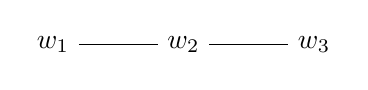
\begin{tikzpicture}[>=stealth']
{[start chain]
\node[on chain] (A) {$w_1$};
\node[on chain,join=by {-},right=of A] (B) {$w_2$};
\node[on chain,join=by {-},right=of B] (C) {$w_3$};}
\end{tikzpicture}
\end{center}
\end{figure}

It's entirely possible that $w_1$ might have conflicts with the rules of $w_3$. During the worlds transfer, $w_1$ would not get the action ledger from $w_3$. Completely illegal action could have been committed in $w_3$ (eg. free money). In this case $w_1$ can required an Action \textbf{Action Ledger Traceback}(\ref{ALT}).

\subsection{Action Ledger traceback}
\label{ALT}
Depending on the required security of a world, an Action Ledger Traceback (ALT) may be requested upon a world transfer. If this is requested, the player must provide a list of action ledgers that date back to either the player genesis or to the last entry of the world committing the audit. The world then needs to obtain $h_s{AL(P_k, w_{k:n})}$ from $w_k$ to $w_n$. If the hashes match then the players history has been confirmed. 
\\\\
It's still entirely possible for the $AL(P_k, w_{k:n})$ to contain actions considered illegal by the world doing the audit. In this case the rewards and actions committed in the offending world are neglected in the world. An ALT should not often return illegal actions as it will result in \textbf{Action Ledger Fragmentation} (\ref{ALF}), if this is seen often the world should consider a disconnect from the offending world. 

\subsection{World Disconnects}
\label{WD}
It's possible a world may issue a disconnect of an adjacent world, this means that players may no longer travel between these worlds. This could leave players orphaned in the disconnected world. It would be logical for the world that issued the disconnect to accept \textbf{refugee packages} (\ref{RP}) from the orphaned player. The history of that player is now forked into two separate paths as the player will still be able to play on either worlds. It would be highly risky for the player to play on both accounts as it could risk an \textbf{action ledger conflict}(\ref{ALC})

\subsection{Action Ledger Conflicts}
\label{ALC}
Figure \ref{fALC} depicts a possible scenario in which $w_2$ disconnects from $w_3$ and $w_5$. If a player resides in $w_{3:5}$ there is now no way to return to $w_{1:2}$. It's possible that these worlds may accept a refugee package and reinstate the player. The player now has the option to play on either forks. In the event of a future path creation between $w_{3:5}$ and $w_{1:2}$ it is possible that that player forks might collide.

\begin{figure}
\caption{Action Ledger Conflict}
\label{fALC}
\begin{center}
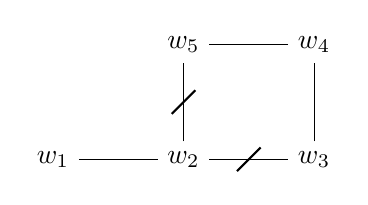
\begin{tikzpicture}[>=stealth']
{[start chain]
\node[on chain] (A) {$w_1$};
\node[on chain,join=by {-},right=of A] (B) {$w_2$};
\node[on chain,join=by {-},right=of B] (C) {$w_3$};
\node[on chain,join=by {-},above=of C] (D) {$w_4$};
\node[on chain,join=by {-},above=of B] (E) {$w_5$};}
\draw[-] (B) -- (E);
\coordinate (MidWay) at ($(B.east)!0.5!(C.west)$);
\draw [thick,-] ($(MidWay)-(\StrikeThru)$) -- ($(MidWay)+(\StrikeThru)$);
\coordinate (MidWay2) at ($(B.east)!0.5!(E.west)$);
\draw [thick,-] ($(MidWay2)-(\StrikeThru)$) -- ($(MidWay2)+(\StrikeThru)$);
\end{tikzpicture}
\end{center}
\end{figure}

This is called an action ledger conflict, and I don't what what to do about it right now...

% \node (WS)[myblock,above of=WE, yshift=1cm]{Worlds Server};

\subsection{One Way Gates}
Worlds can only control their adjacent neighbors, they have no way of controlling the neighbors of their neighbors. Consider Figure \ref{ThreeW}, $w_1$ might have serious issues with $w_3$. There are three ways of dealing with this. The first is to issues a disconnect from $w_2$, this has the disadvantage of players now not being able to travel to $w_2$. The second is to use negotiation tactics with either $w_3$ or $w_2$ to change the rules or disconnect respectively. The third way to is implement a one-way-gate. This is a method of ensuring that illegal rules don't make their way into the issuing world. If $w_1$ issues a one-way-gate against $w_3$ player are no longer allowed to travel back into $w_1$ if they have traveled through $w_3$.

\subsection{World Economic Caps}
It's possible that worlds may require neighboring worlds to employ a \textit{world economic cap}. This sets a hard cap to the amount of resources that can be distributed to players from the environment in a given time period. This can cap experience points, coins, items, etc...

\subsection{Beyond}
The mechanics above are simply suggestions. It's possible for worlds to follow all, some or none of them. Worlds can make their own mechanics. The Worlds Engine is completely open for anyone to modify. Sections of the game might be built on anarchy, others built on peace and justice. There will probably not be a connection between sections like this, which is perfectly fine.

\section{Action Listing} %Why is there a space here?!
\subsection{Construct}
An \textit{action listing} is a data construct containing possible player actions. It's possible for a world to make their own action listing, defining an unlimited amount of possible player actions. World reactions are also reside on this list and start at address code: \textit{0x7F}. There are three types of actions. \textbf{Legal Actions} are action that a world will accecpt into a players action ledger if presented, they reside in the worlds action listing. \textbf{Acceptable Actions} are action that are to be performed in other worlds only, results from these actions are respected. \textbf{Illegal Actions} are actions that a world does not consider to be fair. Illegal actions will simply not show up on a worlds action listing. Action ledger tracebacks (\ref{ALT}) can deal with the occurrence of illegal actions on players action ledgers. 

\begin{figure}
\caption{Section of an Action Listing}
\label{CodeAL}
\lstinputlisting[firstline=1,lastline=13]{../toolkit/ActionListing.yaml}
\end{figure}

\subsection{Action Listing Translation}
As it is possible for worlds to share the exact same action listing, it's possible there might be discrepancies. An action listing translation is a data construct used to translate actions from one worlds actions listing to another worlds action listing.

\section{System Architecture}
\begin{center}
\begin{tabular}{r l}
$A$: & Action\\ 
$Cy(A)$: & Encrypted Action\\
$R$: & Response\\ 
$Cy(R)$: & Encrypted Response\\

\end{tabular}
\end{center}

\begin{small}
\tikzset{myblock/.style = {rectangle, draw, minimum height=1cm, minimum width=3cm}}
\begin{center}
\begin{tikzpicture}
\node(WE)[myblock]{\textbf{Worlds Engine}};
\node (WS)[myblock,above of=WE, yshift=1cm]{Worlds Server};
\node (WC)[myblock,left of=WE, xshift=-3cm, align=center]{Worlds Client};
\node (Key)[myblock,below of=WE, yshift=-1cm]{RSA Key Pair};
\node (AL)[myblock,right of=Key, xshift=3cm]{Action Ledger};
\node (AList)[myblock,left of=Key, xshift=-3cm]{Action Listing};

\draw[->] ($(WE.north east)!0.25!(WE.north west)$) -- node[anchor=west]{$Cy(A)$} ($(WS.south east)!0.25!(WS.south west)$);
\draw[<-] ($(WE.north east)!0.75!(WE.north west)$) -- node[anchor=west]{$Cy(R)$} ($(WS.south east)!0.75!(WS.south west)$);
\draw[->] (WC) -- node[anchor=north]{$A$} (WE);
\draw[<-] (WE) -- (Key);
\draw[<->] (AList) -- (WC);
\draw ($(AList.north east)!0.25!(AList.north west)$)edge[out=90,in=-90,->]($(WE.south east)!0.75!(WE.south west)$);
\draw ($(AL.north east)!0.5!(AL.north west)$)edge[out=90,in=-90,<->]($(WE.south east)!0.25!(WE.south west)$);

% more arrows here
\end{tikzpicture}
\end{center}
\end{small}

\section{Outstanding Issues}
\subsection{Action Ledger Fragmentation}
\label{ALF}
Action ledger fragmentation is when a significant portion of a players action ledger has become 'neglected' due to worlds with action disagreements. 

\subsection{Malicious Worlds}
It's possible for worlds to turn evil, where players would have no recourse traditionally. In this system, since players keep a copy of their action ledger and signed reactions. It's possible to recover from an attack.   

\subsection{World Outages}
In the event of a server outages players may become stranded. The first line of defense for this should be server mirrors. Worlds should run an maintain mirrors that will pickup the slack in the event of an outage. Even if it's a far less capable system, player will at least be able to exit. In the even of a permanent world outage, adjacent worlds should accept signed \textbf{refugee packages}(\ref{RP}).  


\end{document}
